\section{Pictures of Baek's argument}\label{app:baek}

The figures of this appendix illustrate the notions and the steps of Baek's
proof described in \cref{sec:baek}.

\begin{figure}[htbp]
  \centering
  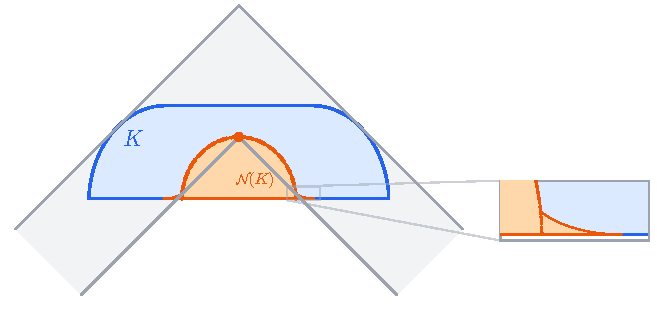
\includegraphics[width=\linewidth]{figures/fig-capniche}
  \caption{Gerver's cap $K$, the union of the blue and the orange regions, and
  its niche $\cN(K)$ (orange); the sofa $\Gs=K\setminus\cN(K)$ is the blue
  region. Grey: the copy of the hallway at the angle $t=\pi/4$. Its outer walls
  touch $K$, and its inner corner (orange dot) lies on the dashed curve, the
  path of the inner corner of the copies as $t$ runs from $0$ to $\pi/2$. Near
  its two ends the niche extends beyond this path, down to the floor, where the
  inner walls, not the corner, touch the sofa; the inset magnifies the right
  end, and the left end is its mirror image.}
  \label{fig:capniche}
\end{figure}

\begin{figure}[htbp]
  \centering
  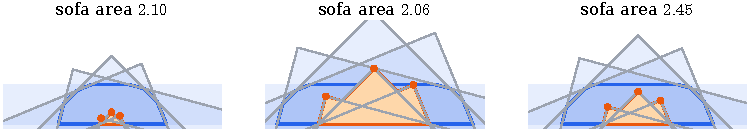
\includegraphics[width=\linewidth]{figures/fig-placements}
  \caption{Three placements of copies of the hallway at the same three angles
  $t=\pi/8,\pi/4,5\pi/12$ (orange dots: their inner corners). Each copy shades
  in light blue the region inside its two outer walls, and so do the start and
  end positions, which keep the sofa in the strip $0\le y\le1$; the polygonal
  cap, outlined in blue, is the darkest region, where all of them overlap, and
  the polygonal niche (orange) is the part of the cap beyond both inner walls of
  at least one copy. Left: copies close in give a small cap. Middle: copies far
  out give a large cap, but also a large niche. Right: a maximum polygon cap for
  these angles.}
  \label{fig:placements}
\end{figure}

\begin{figure}[htbp]
  \centering
  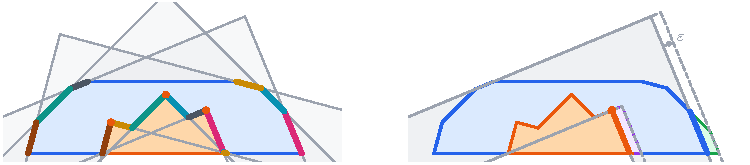
\includegraphics[width=\linewidth]{figures/fig-balance}
  \caption{Balance of the maximum polygon cap of \cref{fig:placements}. Left:
  the three copies of the hallway (light grey; orange dots: their inner
  corners); each slanted side of the cap lies on an outer wall of one of the
  copies, and is drawn thick in the same colour as the side of the niche on the
  inner wall of the same copy parallel to it; the two have the same length. A
  side of the niche may consist of several pieces, as for the amber pair. Right:
  Gerver's balancing argument. The copy at the angle $\pi/8$ (light grey) is
  moved outward by $\eps$ (dashed), which moves one of its outer walls and the
  inner wall parallel to it and leaves the other two walls in place. This adds
  to the cap a strip along its side on that wall (green), and to the niche a
  strip along its side on the inner wall (purple); the two sides are drawn
  thick. The sofa area changes by about $\eps$ times the difference of their
  lengths, so if they differed, moving the walls outward or inward would
  increase it; here the two sides have the same length, $0.63$, as they do at
  each of the six slanted sides of this cap.}
  \label{fig:balance}
\end{figure}

\begin{figure}[htbp]
  \centering
  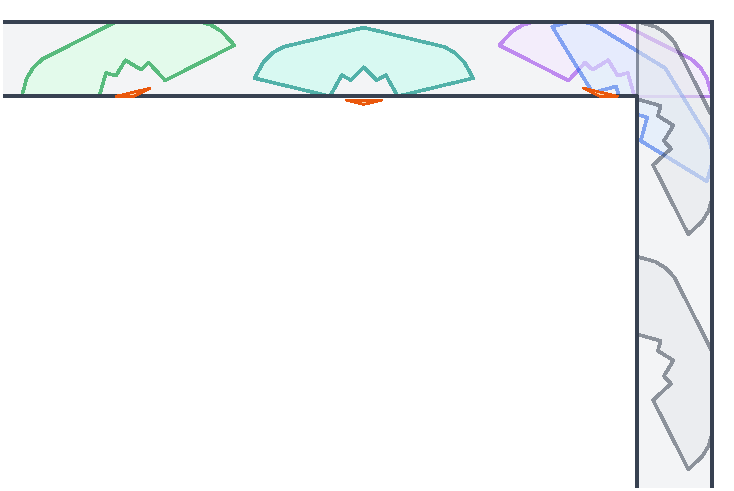
\includegraphics[width=\linewidth]{figures/fig-turn}
  \caption{Step (3a) for an actual sofa: a polygonal cap with rotation angle
  $\omega=1.1$ (about $63^\circ$) minus its niche. A copy of the sofa turned by
  $\pi/2-\omega$ (green) first turns back inside the horizontal side, before the
  corner, through the position halfway (teal), to the sofa's own starting
  position (purple). This is possible because the small triangle at the inner
  corner (orange) lies in the hollow of the sofa, which keeps its height at most
  $1$ throughout this turn. The copy then follows the sofa's own movement and
  turns by $\omega$ around the corner (blue halfway, grey at the end, and again
  slid down the vertical side). In total, it turns by the full right angle.}
  \label{fig:turn}
\end{figure}

\begin{figure}[htbp]
  \centering
  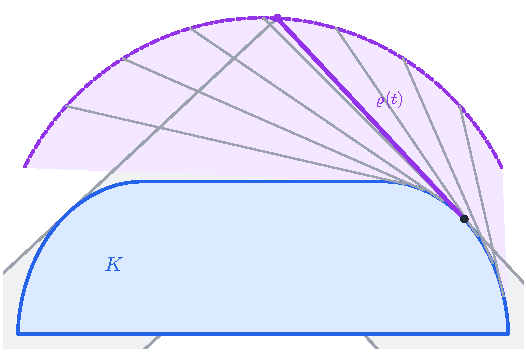
\includegraphics[width=0.75\linewidth]{figures/fig-mamikon}
  \caption{One of the terms of $\cQ$ in step (4), for Gerver's cap $K$. For an
  angle $t$, the segment of length $\varrho(t)$ runs along an outer wall of the
  copy of the hallway at the angle $t$, from the point where $K$ touches that
  wall (black dot) to the outer corner of the copy (purple dot); the copy at the
  angle $t$ is drawn in light grey, with its two outer walls touching $K$. The
  thin grey segments are the same segment for other angles. As $t$ runs from
  $\varphi$ to $\pi/2-\varphi$, where $\varphi=0.039\ldots$ is Gerver's angle
  (Appendix~\ref{app:gerver}) and this is the range of angles in which the inner
  corner of the hallway touches Gerver's sofa, the segment sweeps the shaded
  region, whose area is $\frac12\int\varrho(t)^2\dd t$ by Mamikon's theorem; the
  dashed curve is the path of the outer corner.}
  \label{fig:mamikon}
\end{figure}
